\section*{Method}
\label{Method}
%
The method of choice in this paper is Principal Component Analysis (PCA). This method is typically used as an explorative technique to obtain an overview by reducing a complex data set to a lower number of dimensions. The dimensions found in PCA is called principal components (PC). Each PC explains a certain amount variation noted in percentage which describes how much of the variances of the original variables, the PC describes.\blankline
%
PCA uses linear algebra to extract the components. The PCA consists of different steps, an overview of these different steps is listed based on \textcite[pp. 211-213]{Naes2010}:

\begin{enumerate}
	\item Organise the data in a data matrix where each row in the table corresponds to an ‘object’ and each column to a ‘variable’
	\item Computing the average of all the variables. 
	\item The averages are subtracted from their corresponding variables.
	\item Search for the direction in space that has as large variance as possible, which is the first principal component (PC1).
	\item Search for the second principal component(PC2). Same procedure as for PC1, but under the restriction that the direction of the PC2 is orthogonal to PC1. 
	\item Extract new components that describe as much variance as possible under the restriction that each new PC-direction is orthogonal to the previous.
	\item Stop extraction when the desired number of components have been extracted. In many cases 2-3 components is enough to explain most of the variation. 
\end{enumerate}
\blankline
%
The variances of each PC is noted in percentage.
The sum of the variances of the PC's is equal to the sum of the variances of the original variables. This means that if we have two components, the sum of this two components describes the total percentage covered be them. An example could be PC1 = 87 \% and PC2 = 9 \%. The total variances covered be having two components in this case will be 87 \% + 9 \% = 96 \% \parencite[p. 213]{Naes2010}. This could be useful when determine when the desired number of components has been extracted. \blankline
%
Score value is the principal component value 
Loading values defines the contribution of each of the original variables in the calculation of the first score. This means that a high loading value for a specific variable indicates that this variable is strongly related to the PC, that the loading value is according to. 

The results of the PCA is typically presented graphically in a scatter plot in two- or three-dimensions, where each dimension is based on a PC. This plot is called score plot. An example of a score plot in two dimensions is presented in \autoref{fig:PlotExample}
%
\begin{figure}[H]
\centering
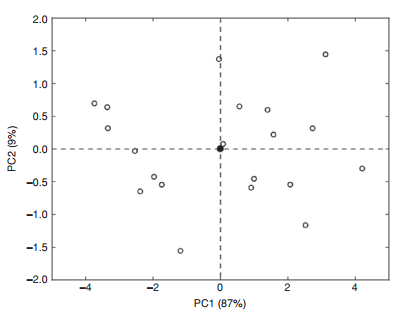
\includegraphics[width =0.7\textwidth]{Figure/PlotExample}
\caption{Example of two-dimension score plot \parencite[p. 215]{Naes2010}.}
\label{fig:PlotExample}
\end{figure}
\noindent
%
The scores plot is therefore simply a plot of the relation between the objects in the projected space.